\documentclass{article}
\usepackage{ctex}
\usepackage{bm}
\usepackage{tikz}
\usepackage{amsmath}
\usepackage{graphicx}
\usepackage[a4paper, margin=3.5cm]{geometry}
\renewcommand{\baselinestretch}{1.5} 
\begin{document}
\section{世界的舞台: 场方程}
\subsection{潮汐力与测地偏离}

你也许听说过:在太空中自由下落的宇航员是\textbf{失重}的。他们感觉不到重力,就像它从未存在一样。但如果重力真的“消失”了,那我们还剩下什么?爱因斯坦敏锐地指出:自由落体并不意味着没有引力,它只是以一种新的方式留下了痕迹。

想象你穿着宇航服,漂浮在距离地球一定高度的空间中。这次你不在空间站里,而是一个人悬停在太空中,靠喷气背包保持静止。你脚下是地球,头顶是无边宇宙。此刻,围绕你布满了均匀分布的金属小珠子,构成一个球形壳体,每颗珠子都和你一样静止。

现在,你关闭喷气背包,和这些珠子一起开始自由下落,朝向地球坠落。最初,你感觉不到任何特别之处,所有的珠子似乎都安静地围绕着你。毕竟\textbf{如果地球的引力场是完全均匀的,那你们的加速度将完全一致},相对距离也完全不会发生改变。

但渐渐地,事情开始变化。你会发现球壳赤道上的珠子,也就是你身边水平方向的珠子,开始缓慢地向你靠近。而头顶和脚下的珠子却慢慢地远离你。原来本各向同性的球面变得越来越椭。
\begin{figure}[h]
    \centering
    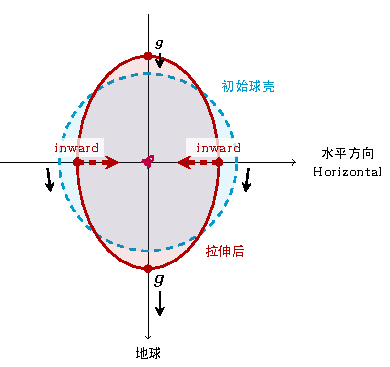
\includegraphics[scale=1.2]{./tikz/fig1.pdf}
\end{figure}

这正是引力场不均匀的表现:你和身边的珠子都在加速,但你们加速的方向都指向地球中心,因此轨迹在会聚——水平上的珠子看起来正靠近你。另一方面,你脚下的珠子离地球更近,它比你受到更强的引力,因此加速更快,从你视角看,它向下远去;而你头顶的珠子离地球更远,它加速得没你快,因此也逐渐被你甩在身后。

这种在某些方向上拉伸、在另一些方向上压缩的引力效应,就是著名的\textbf{潮汐力}。它并不是引力本身,而是引力场变化留下的痕迹。

你可能会问:如果我们不是从静止状态掉下去,而是以恰好合适的速度水平飞行,绕地球做一个圆形轨道呢?结果是一样的。你和那一球珠子仍然会受到同样的潮汐力。

接下来我们从牛顿引力出发,一步步从潮汐力走向场方程。

\subsubsection{牛顿引力下潮汐力的几何特征}

想象一下,假设最初的粒子球体被封闭在一个立方体中。当球体下落并变形为椭球时,封闭的立方体及其内容物会发生线性变换,将其变形为一个边长为 $2\xi, 2\zeta$ 和 $2\Xi$ 的盒子,因此体积为 $8\xi\zeta\Xi$。注意到对于水平方向,$\xi$与$\zeta$的地位应当是等价的,且鸡蛋所占的体积是这个盒子的一个固定比例,我们有:
\begin{equation}
\delta \mathcal{V} = \frac{4\pi}{3} \xi^2 \Xi\label{1.1.1.1}
\end{equation}

由于你和粒子球从静止开始,显然这个体积的变化率最初为零:$\delta \dot{\mathcal{V}} = 0$。这可以通过计算来验证:
\begin{align*}
\delta \dot{\mathcal{V}} &= \frac{4\pi}{3} \left[ 2\xi \dot{\xi} + \xi^2 \dot{\Xi} \right] = 0
\end{align*}

但是潮汐力会立即加速球体的粒子,所以现在让我们计算鸡蛋体积的二阶导数:
\begin{align*}
\delta \ddot{\mathcal{V}} &= \frac{4\pi}{3} \left[ 2(\dot{\xi})^2 + 2\xi \ddot{\xi} + 2\dot{\xi} \dot{\Xi} + \xi^2 \ddot{\Xi} \right] \\
&= \frac{4\pi}{3} \left[ 2\xi \ddot{\xi} + \xi^2 \ddot{\Xi} \right]
\end{align*}

但是,最初 $\xi = \delta r = \zeta$,且水平方向的引力差和垂直方向的引力差分别控制,因此:
\begin{align*}
\delta \ddot{\mathcal{V}} &= \frac{4\pi}{3} \left[ 2\delta r \ddot{\xi} + \delta r^2 \ddot{\Xi} \right] = \frac{4\pi}{3} (\delta r)^2 \left( 2\mathcal{K}_+ + \mathcal{K}_- \right) \\
&= {0}
\end{align*}
其中$\mathcal K_{\pm}$由以下两个公式确定:
\begin{gather*}
    \ddot{\xi} = -\mathcal{K}_+ \xi \quad \Rightarrow \quad \mathcal{K}_+ = +\frac{GM}{r^3}\\
    \ddot{\Xi} = -\mathcal{K}_- \Xi \quad \Rightarrow \quad \mathcal{K}_- = -\frac{2GM}{r^3}
\end{gather*}

由$\delta\ddot{\mathcal V}=\delta\dot{\mathcal V}=0$,我们可以得到美丽的平方反比潮汐力的几何特征:由平方反比定律产生的潮汐力、且只有平方反比定律是\textbf{保持体积}的。

\subsubsection{牛顿引力下吸引力的几何特征}

在前面的分析中,我们暂时忽略了球壳内部粒子对彼此的引力影响。但实际上,如果你从球体中被移开,并将原本你所在位置填充为密度为 $\rho$ 的致密物质,它将对其余粒子产生新的引力源。

假设粒子球半径为 $\xi = \Xi$,此时球体内的粒子将受到这块致密物质的吸引。等效地,可以认为中心存在一团质量为 $\rho \, \delta \mathcal{V}$ 的物质,产生引力使粒子向中心加速:
\begin{equation*}
\ddot{\xi} = -\frac{G \rho \, \delta \mathcal{V}}{\xi^2}
\end{equation*}
现在我们来计算这种情况下鸡蛋体积的加速度。根据\eqref{1.1.1.1}:
\begin{equation*}
\delta \mathcal{V} = \frac{4\pi}{3} \xi^3
\end{equation*}
我们对其进行两次时间导数,有:
\begin{align*}
\dot{\delta \mathcal{V}} &= 4\pi \xi^2 \dot{\xi} \\
\ddot{\delta \mathcal{V}} &= 8\pi \xi \dot{\xi}^2 + 4\pi \xi^2 \ddot{\xi}
\end{align*}

由于初始时 $\dot{\xi} = 0$,上式简化为:

\begin{equation*}
\ddot{\delta \mathcal{V}} = 4\pi \xi^2 \ddot{\xi} = 4\pi \xi^2 \left( -\frac{G \rho \, \delta \mathcal{V}}{\xi^2} \right) = -4\pi G \rho \, \delta \mathcal{V}
\end{equation*}

因此我们得到了一个非常优雅的结论:
\begin{equation}
    \ddot{\delta \mathcal{V}} = -4\pi G \rho \, \delta \mathcal{V}
\end{equation}
即:对于一个填充了密度为 $\rho$ 物质的球体而言,其体积的加速度正比于它本身,且符号为负,表示球体会向内坍缩。这种行为是平方反比引力的直接体现,体现了其稳定、集中的吸引性质。


\end{document}